\section{Results}
\paragraph{Gamma spectra?}
The spectra were obtained

[Calibration] was then necessary,
in order [to derive the linear relationship] between [the channels] of the Multi Channel Analyser (MCA) thingy in which signal is detected 
and the corresponding energy values.
This was accomplished using the known decay schems of the four sources.
\begin{figure}[htbp]
    \centering
    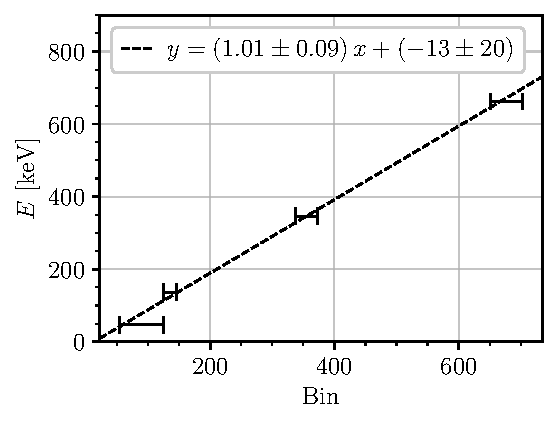
\includegraphics[scale=1]{figures/calibration_energy.pdf}
    \caption{Calibration}
    \label{fig:calibration_energy}
\end{figure}
\paragraph{Statistics}

\begin{figure}[htbp]
    \centering
    \begin{subfigure}{0.495\textwidth}
        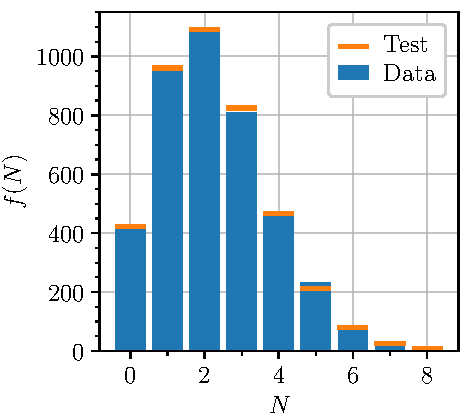
\includegraphics[scale=1]{figures/lowmean_poisson.pdf}
    \end{subfigure}
    \begin{subfigure}{0.495\textwidth}
        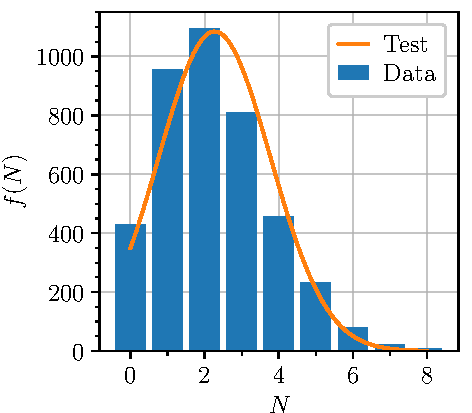
\includegraphics[scale=1]{figures/lowmean_gaussian.pdf}
    \end{subfigure}
    \begin{subfigure}{0.495\textwidth}
        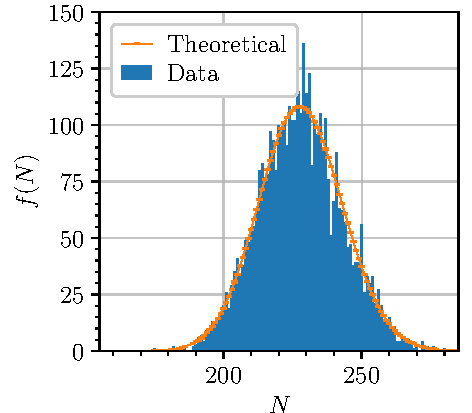
\includegraphics[scale=1]{figures/highmean_poisson.pdf}
    \end{subfigure}
    \hfill
    \begin{subfigure}{0.495\textwidth}
        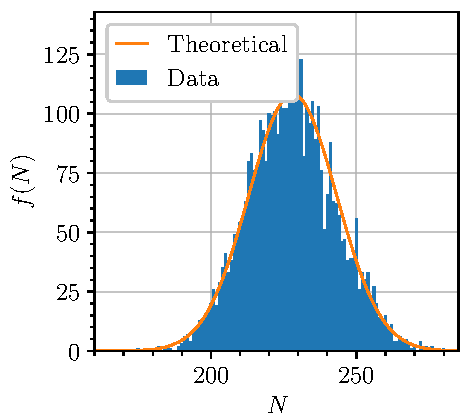
\includegraphics[scale=1]{figures/highmean_gaussian.pdf}
    \end{subfigure}
\end{figure}

\paragraph{Attenuation [in matter?]}
[We chose Cesium because of its high count rate]

The linear attenuation coefficient was found to be $\mu = (0.20 \pm 0.01)$ \unit{\per\cm} for Aluminium
and $\mu = (1.08 \pm 0.03)$ \unit{\per\cm} for Lead.
\begin{figure}[htbp]
    \centering
    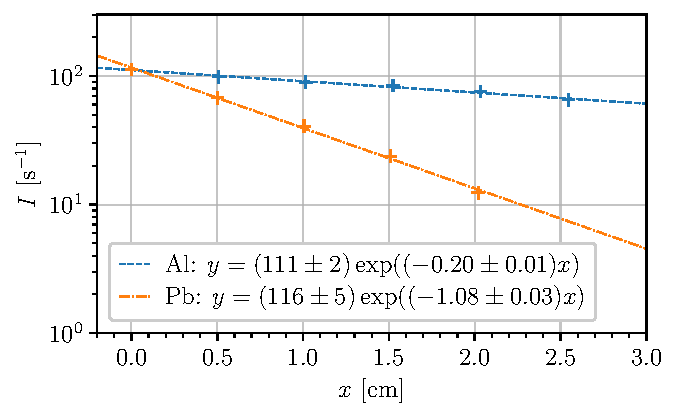
\includegraphics[scale=1]{figures/attenuation_coefficient.pdf}
    \caption{Radiation attenuation through Aluminum (Al) and Lead (Pb). 
             The error bars were omitted in reason of their small relative size 
             (1\% on the intensity and $1$ $\mu$m on the thickness of the material).}
    \label{fig:attenuation_coefficient}
\end{figure}

\paragraph{À METTRE DANS DISCUSSION}
After obtaining the linear attenuation coefficient it was possible to derive the energies of the $\gamma$ rays emitted from the source by checking the tables contained in Annex D of \cite{notice_generale}.
These indicate a corresponding energy of $\approx 0.7$ MeV for both materials.
\hl{maybe faut etre plus clairs sur qu'est-ce que ca contient la table}

The results are compatible with the previously obtained [or known??] spectrum for the $^{137}$Cs